\documentclass[12pt, a4paper]{article}

\usepackage[utf8]{inputenc}
\usepackage[english, russian]{babel}
\usepackage{fancyhdr}
\usepackage{amsmath}
\usepackage{amsthm}
\usepackage{float}
\usepackage{graphicx}
\graphicspath{ {./} }
\usepackage{tabularx}
\newcolumntype{L}{>{\raggedright\arraybackslash}X}
\usepackage{pgfplots}
\usepackage{float}
\usepackage{xcolor}
\usepackage{hyperref}
\usepackage{multirow}
\usepackage{diagbox}
\pgfplotsset{width=\textwidth*0.8, compat=1.13}

\usepgfplotslibrary{external}
\usepgfplotslibrary{fillbetween}
\usepgfplotslibrary{statistics}
\usetikzlibrary{patterns.meta}


\graphicspath{{./}}
\newcommand{\Mod}[1]{\ \mathrm{mod}\ #1}

\usepackage[a4paper, margin=1.5cm]{geometry}

\usepackage{titlesec}
\titlelabel{\thetitle.\quad}

\pagestyle{plain}

\fancypagestyle{firstpage}{%
  \chead{
  МИНИСТЕРСТВО НАУКИ И ВЫСШЕГО ОБРАЗОВАНИЯ РОССИЙСКОЙ ФЕДЕРАЦИИ 
ФЕДЕРАЛЬНОЕ ГОСУДАРСТВЕННОЕ АВТОНОМНОЕ  
ОБРАЗОВАТЕЛЬНОЕ УЧРЕЖДЕНИЕ ВЫСШЕГО ОБРАЗОВАНИЯ\bigskip

«Национальный исследовательский университет ИТМО»\bigskip

ФИЗИЧЕСКИЙ ФАКУЛЬТЕТ 
}
\fancyfoot[CO]{Санкт-Петербург, 2023}%
}



\definecolor{aqua}{HTML}{003844}
\definecolor{peri}{HTML}{5EB1BF}
\definecolor{royal_blue}{HTML}{0A2463}
\definecolor{periwinkle}{HTML}{D8DCFF}
\definecolor{cerulean}{HTML}{247BA0}
\definecolor{bloodred}{HTML}{690500}
\definecolor{imperial_red}{HTML}{FB3640}
\definecolor{purple}{HTML}{511730}
\definecolor{tangerine}{HTML}{FFA781}

\definecolor{blue1}{HTML}{142459}
\definecolor{blue2}{HTML}{176BA0}
\definecolor{blue3}{HTML}{19AADE}
\definecolor{blue4}{HTML}{1AC936}
\definecolor{blue5}{HTML}{1DE4BD}
\definecolor{blue6}{HTML}{6DF0D2}

\definecolor{pink1}{HTML}{29066B}
\definecolor{pink2}{HTML}{7D3AC1}
\definecolor{pink3}{HTML}{AF4BCE}
\definecolor{pink4}{HTML}{DB4CB2}
\definecolor{pink5}{HTML}{EB548C}
\definecolor{pink6}{HTML}{EA7369}
\newtheorem*{task}{Условие}
\newtheorem*{finish}{Заключение}

\counterwithin{figure}{section}

%\tikzexternalize
\begin{document}
\newgeometry{top=1.6cm,bottom=1.6cm, left = 1.2cm, right = 1.2cm}

\topskip0pt
\vspace*{0.25\textheight}
\begin{center}
\textbf{\LARGE РАБОЧИЙ ПРОТОКОЛ И ОТЧЁТ }

\LARGE по лабораторной работе №3.13

\LARGE <<Магнитное поле Земли>>

\end{center}
\vspace*{5cm}
\begin{flushright}
\begin{minipage}{.33\linewidth}
\textit{\textbf{Выполнил:}}\\
Хороших Дмитрий - P3217\\
\textit{\textbf{Преподаватель:}}\\
Коробков Максим\\ Петрович
\end{minipage}
\end{flushright}


\thispagestyle{firstpage}
\newpage
\tableofcontents

\restoregeometry
\section{Введение}
\begin{enumerate}
\item Цель работы:

Определение горизонтальной составляющей магнитного поля Земли.

\item Задачи:
	\begin{enumerate}
		\item[1.]  Провести измерения направления суммарного магнитного поля, создаваемого Землёй и системой катушек Гельмгольца.
		\item[2.] По полученным измерениям вычислить горизонтальную составляющую магнитного поля Земли.
	\end{enumerate}
		
\item Объект исследования:

Магнитное поле Земли.

\item Экспериментальная установка:
\begin{figure}[H]
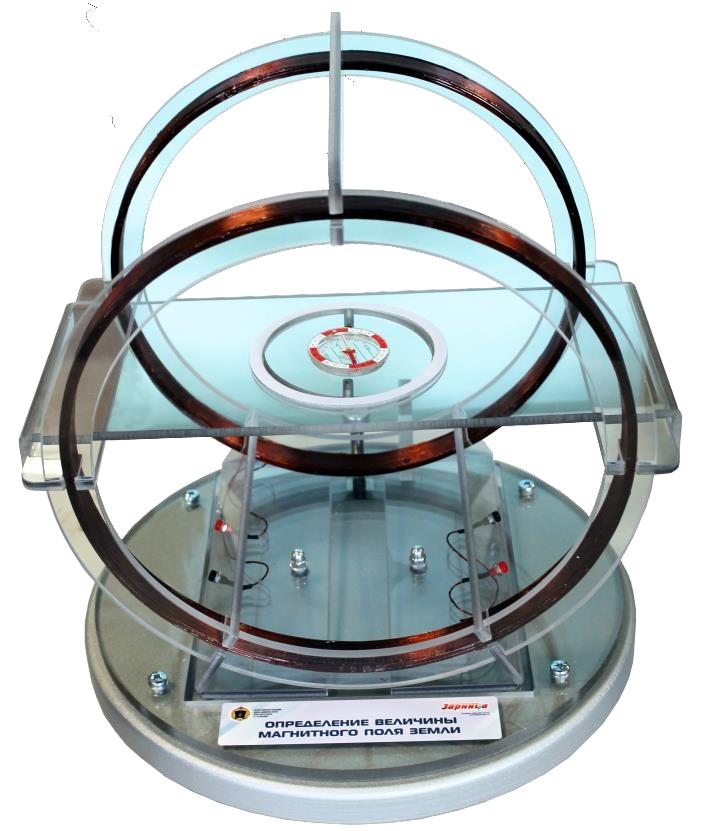
\includegraphics[width=0.5\textwidth]{../helmholtz.png}
\centering
\caption{Экспериментальная установка - Кольца Гельмгольца}
\end{figure}

Состоит из 2-х колец Гельмгольца, источника тока с амперметром и компаса с круговой транспортирной сеткой.

\item Метод экспериментального исследования:

Многократный прямой замер.

\item Рабочие формулы:

Магнитная индукция на оси колец Гельмгольца в точке, равнотстоящей от обеих обмоток:
\begin{equation}
B = \mu_0 (\frac{4}{5})^{\frac{3}{2}} \frac{I n}{R}
\end{equation}

Связь магнитной индукции, создаваемой установкой, с горизонтальной составляющей магнитного поля Земли:
\begin{equation}
B_c = B_h \cdot \frac{\sin(\alpha)}{\sin(\varphi - \alpha)}
\end{equation}



\item Измерительные приборы:

\begin{table}[H]
\centering
\begin{tabular}{|l|l|l|l|l|}
\hline
№ п/п & Наименование & Тип & Используемый диапазон & Погрешность приб.\\
\hline
1 & Амперметр & Электронный & -  & 0.05 мА\\
\hline
2 & Транспортирная сетка & Аналоговый & 0-360$^{\circ}$  & 0.5$^{\circ}$\\
\hline
\end{tabular}
\end{table}

\end{enumerate}
\section{Результаты измерений и их обработка}

Установим кольца Гельмгольца так, чтобы их ось составляла с линией магнитной индукции Земли угол $\varphi \simeq 160^{\circ}$.

Подадим ток на кольца и, меняя силу тока, запишем показания амперметра для определённых углов отклонения стрелки компаса $\alpha$:

\begin{table}[H]
\begin{center}
\begin{tabular}{|c|c|c|c|c|c|c|c|}
\hline 
$\alpha_i$ & $I_1$, мА & $I_2$, мА & $I_3$, мА & $I_4$, мА & $\langle I \rangle$, мА & $\frac{\sin(\alpha_i)}{\sin(\varphi - \alpha_i)}$ & $B_c$, мкТл \\ 
\hline 
10$^{\circ}$ & 8.64 & 7.60 & 7.20 & 7.30 & 7.69& 0.35 & 4.61\\ 
\hline 
20$^{\circ}$ & 12.67 & 12.60 & 11.50 & 12.80 & 12.39& 0.53 & 7.43\\ 
\hline 
30$^{\circ}$ & 15.33 & 15.50 & 14.20 & 16.00 & 15.26& 0.65 & 9.15\\ 
\hline 
40$^{\circ}$ & 17.26 & 16.80 & 16.80 & 17.90 & 17.19& 0.74 & 10.30\\ 
\hline 
50$^{\circ}$ & 18.80 & 19.30 & 18.00 & 20.00 & 19.02& 0.82 & 11.40\\ 
\hline 
60$^{\circ}$ & 20.00 & 21.20 & 19.50 & 21.40 & 20.52& 0.88 & 12.30\\ 
\hline 
70$^{\circ}$ & 21.50 & 22.60 & 20.60 & 22.80 & 21.88& 0.94 & 13.11\\ 
\hline 
80$^{\circ}$ & 22.80 & 23.80 & 22.40 & 24.10 & 23.28& 1.00 & 13.95\\ 
\hline 
90$^{\circ}$ & 24.10 & 25.50 & 26.00 & 25.50 & 25.27& 1.06 & 15.15\\ 
\hline 
100$^{\circ}$ & 25.80 & 27.00 & 25.80 & 28.90 & 26.88& 1.14 & 16.11\\ 
\hline 
110$^{\circ}$ & 28.00 & 29.60 & 27.00 & 30.00 & 28.65& 1.23 & 17.17\\ 
\hline 
120$^{\circ}$ & 28.80 & 33.30 & 29.10 & 31.60 & 30.70& 1.35 & 18.40\\ 
\hline 
130$^{\circ}$ & 33.50 & 37.30 & 33.70 & 33.50 & 34.50& 1.53 & 20.68\\ 
\hline 
140$^{\circ}$ & 38.00 & 45.90 & 42.90 & 43.30 & 42.53& 1.88 & 25.49\\ 
\hline 




\end{tabular}
\caption{Результаты прямых измерений силы тока при различных углах отклонения $\alpha_i$ и итоги их обработки.}
\label{tab:1}
\end{center}
\end{table}

Отметим на графике вычисленные на основе экспериментальных данных значения $B_c$ и аппроксимируем линейную зависимость $B_c=B_h (\gamma_i)$, где $\gamma_i = \frac{\sin(\alpha_i)}{\sin(\varphi - \alpha_i)}$, методом наименьших квадратов.

\begin{figure}[H]
\centering
\begin{tikzpicture}
\begin{axis}[
	axis lines = left,
	ylabel = \(B_c \text{, мкТл}\),
	xlabel = \(\gamma\),
	ymin=0,	
	ymax=30,
	xmin=0,
	xmax=2,
	grid=both,
    grid style={line width=.1pt, draw=gray!10},
    major grid style={line width=.2pt,draw=gray!50},
    minor tick num=5,
	axis x line = bottom,
	axis line style ={line width = .3pt},
	legend style={at={(0.05, 0.85)},anchor=west}
	]
\addplot[only marks, blue2, mark size =2pt, mark=square*, error bars/.cd, y dir=both, y explicit, x dir=both, x explicit, error mark options={ blue2,mark size=0.4pt, line width=4pt }, error bar style={fill=blue2,scale=2, line width=1pt}] table [y = B, x = SINS,  col sep=comma] {../b_sin_division.csv}; 
\addplot[blue1, domain=0:2, thick] {13.809504478707701*x}; 

 
\legend{Экспериментальные данные, Линейная аппроксимация $B_c=B_h \cdot \gamma$}

\end{axis}
\end{tikzpicture}
\caption{График зависимости магнитной индукции ($B_c$), создаваемой кольцами Гельмгольца, от величины $\gamma$, характеризующей отклонение стрелки компаса относительно начального положения. }
\label{gr:1}
\end{figure}

Аппроксимируя функцию магнитной индукции $B_c$ прямой, получаем \[ B_c = B_h \cdot \gamma =  13.81\cdot \gamma\]

Таким образом, искомая горизонтальная составляющая магнитной индукции Земли $B_h$ равна:

\[B_h = 13.81 \pm 0.1 \text{, мкТл}\]

Доверительный интервал ($\alpha=0.95$):
\[ B_h \in \left[13.67; 13.95 \right] \text{, мкТл} \]

Табличное значение для горизонтальной составляющей магнитной индукции Земли ($B_h$) для корпуса ИТМО на ул. Ломоносова, Санкт-Петербург 18.04.24 получим при помощи модели Британской Геологической Службы (BGS) - \href{http://www.geomag.bgs.ac.uk/data_service/models_compass/wmm_calc.html }{http://www.geomag.bgs.ac.uk}:

\[B_{h\text{, табл.}} = 14.765 \text{, мкТл}\]

Полученное нами в ходе эксперимента значение $B_h$ отклоняется от $B_{h\text{, табл.}}$ не более чем на $7 \%$.

\newpage

\section{Вывод}
Таким образом, в ходе выполнения лабораторной работы удалось, измерив силу тока, необходимую для создания кольцами Гельмгольца магнитного поля, отклоняющего стрелку компаса на различные углы $\alpha$:

Определить горизонтальную составляющую магнитного поля Земли ($B_h = 13.81 \pm 0.1 \text{, мкТл}$) и сравнить полученное значение с табличным.

\section{Приложение}
Проект этой лабораторной работы, содержащий файлы с Python-кодом, использованным для вычислений и исходные TeX-файлы доступен по - \href{https://github.com/Dimankarp/Studies/tree/main/LaTeX/Physics%20-%20Earth%20Magnetism}{ссылке}.

\end{document}



